\section{Results}\label{sec:results}

\subsection{Base case calculation}
As a reference for all following calculations, a model representing the final design of the Blennerhassett Island Bridge is investigated. The results obtained by the calculations are then compared to the ones in the design drawings for plausibility. A particular challenge is the determination of the self-equilibrium stress state. As the arch was defined as an unsuitable parabola, appropriate hanger forces were determined by trial and error in the design. These permanent hanger forces of the final design are available in the drawings. However, for the calculation of the base case they are unsuitable, as the load distribution in the model is simplified. Instead of another trial and error procedure for the base case, the hanger forces are obtained as the result of a simultaneous arch and tie moment optimisation. Thereby, the moment in the arch is weighed by a factor of 1.5 in order to achieve on optimal similarity. Further, the hanger forces are bounded between 25\% and 45\% of their nominal strength. The internal force distributions of the base case for the permanent state are shown in Fig. \ref{fig:base_case_permanent}. Instead of the normal force in the hangers, the demand over capacity ratio is shown directly. Only the hangers of one set are shown, namely the ones inclined to the right side, and the dots are connected for readability. As a comparison, the extreme values found on the design drawings are also shown.

\begin{figure}[H]
    \centering
    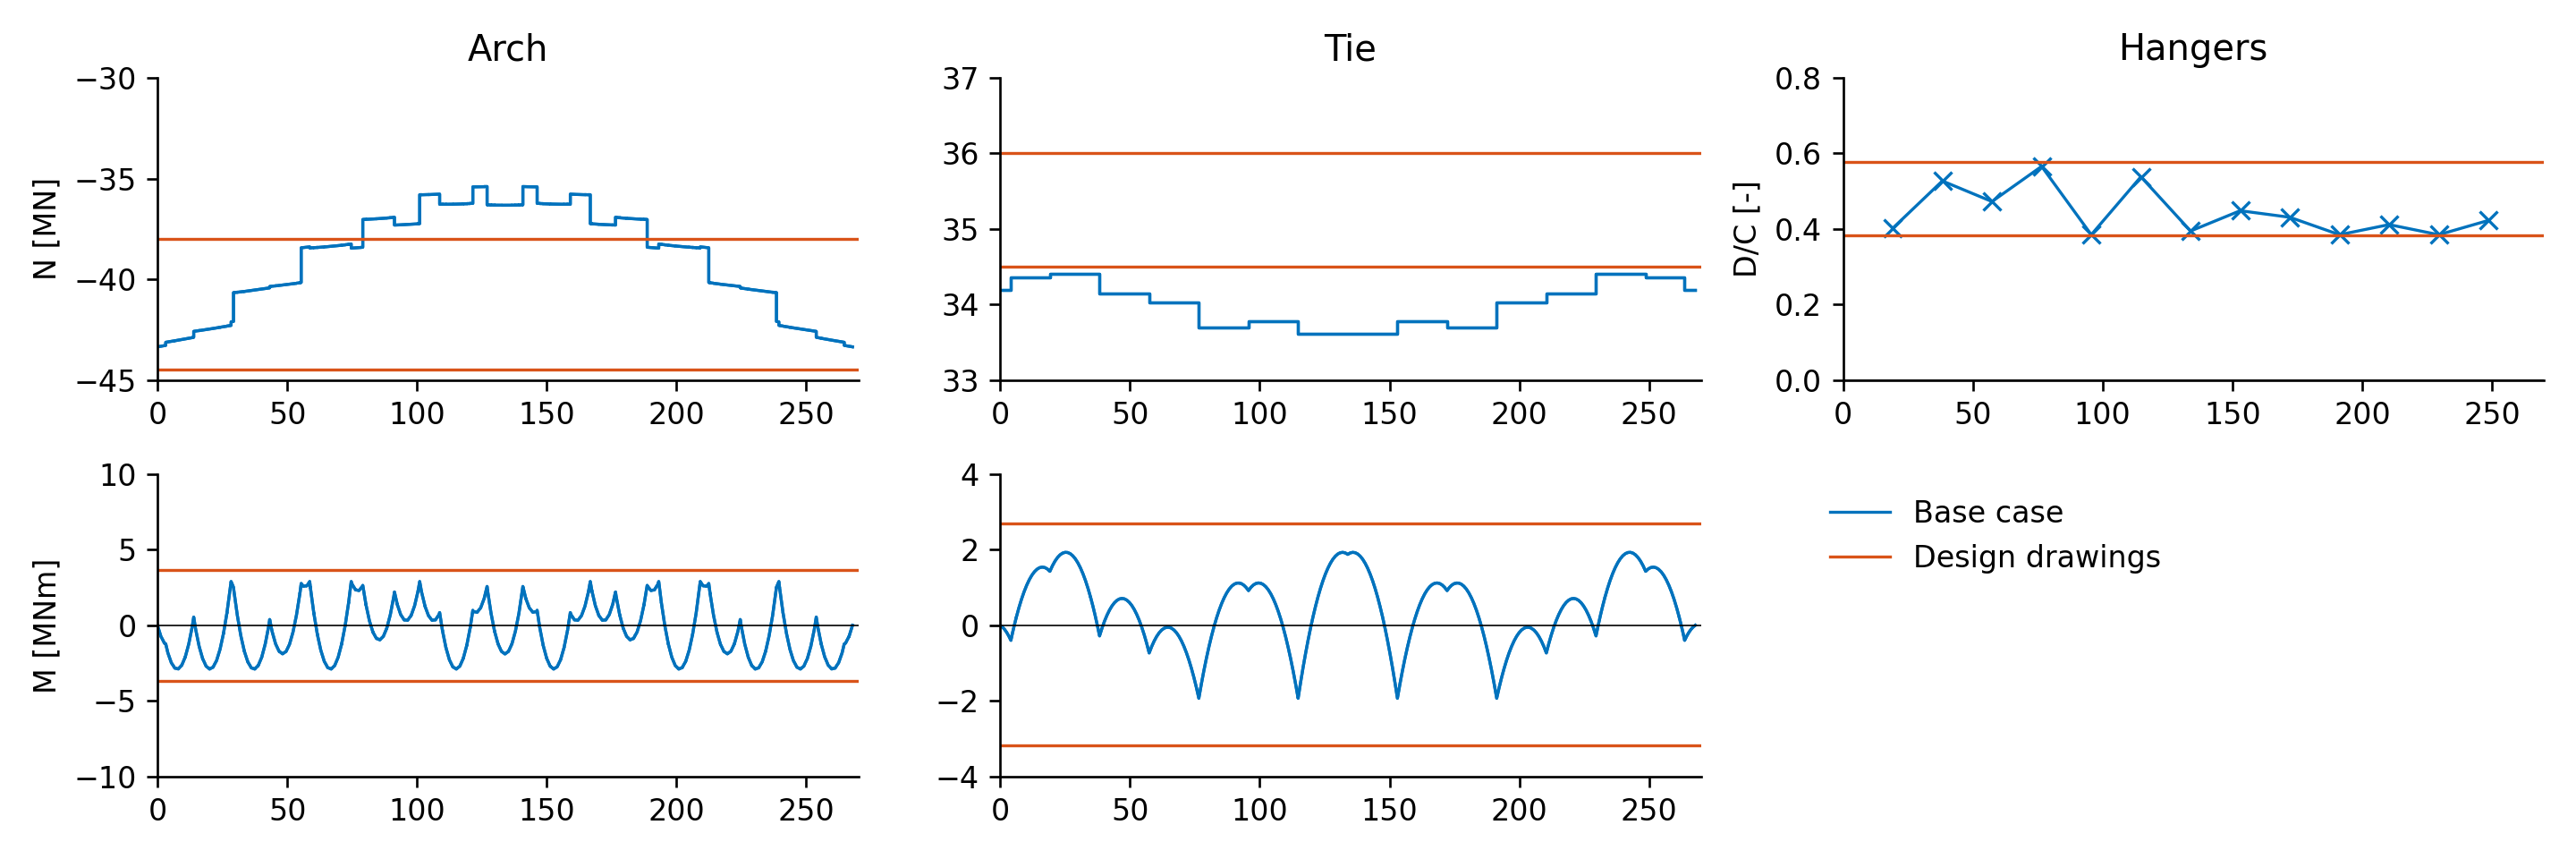
\includegraphics[width=\textwidth]{calculations/Base case/Permanent state.png}
    \caption{Permanent internal forces of the base case and reference values from the drawings}
    \label{fig:base_case_permanent}
\end{figure}

It can be seen, that the moment distributions in the arch and the tie as well as the normal forces in the hangers match the design drawings very well. Only for the normal force in the arch and the tie an offset of \SI{2}{MN} can be observed. This difference is probably due to an underestimation of the weight of the bridge and its simplified assignment to the beams. However, overall the obtained internal force distribution matches the design drawings sufficiently well. It can be concluded, that for a fixed arch shape the simultaneous arch and tie moment optimisation yields adequate results.\medskip

Another comparison is drawn between the effects under characteristic live loads. As there are countless live load combinations, which are to be accounted for, it makes sense to look at the entire ranges of possible internal forces. They are shown in Fig. \ref{fig:base_case_live} by the two blue lines, which represent the lower and the upper limit. They are compared to the extreme values found in the design drawings.

\begin{figure}[H]
    \centering
    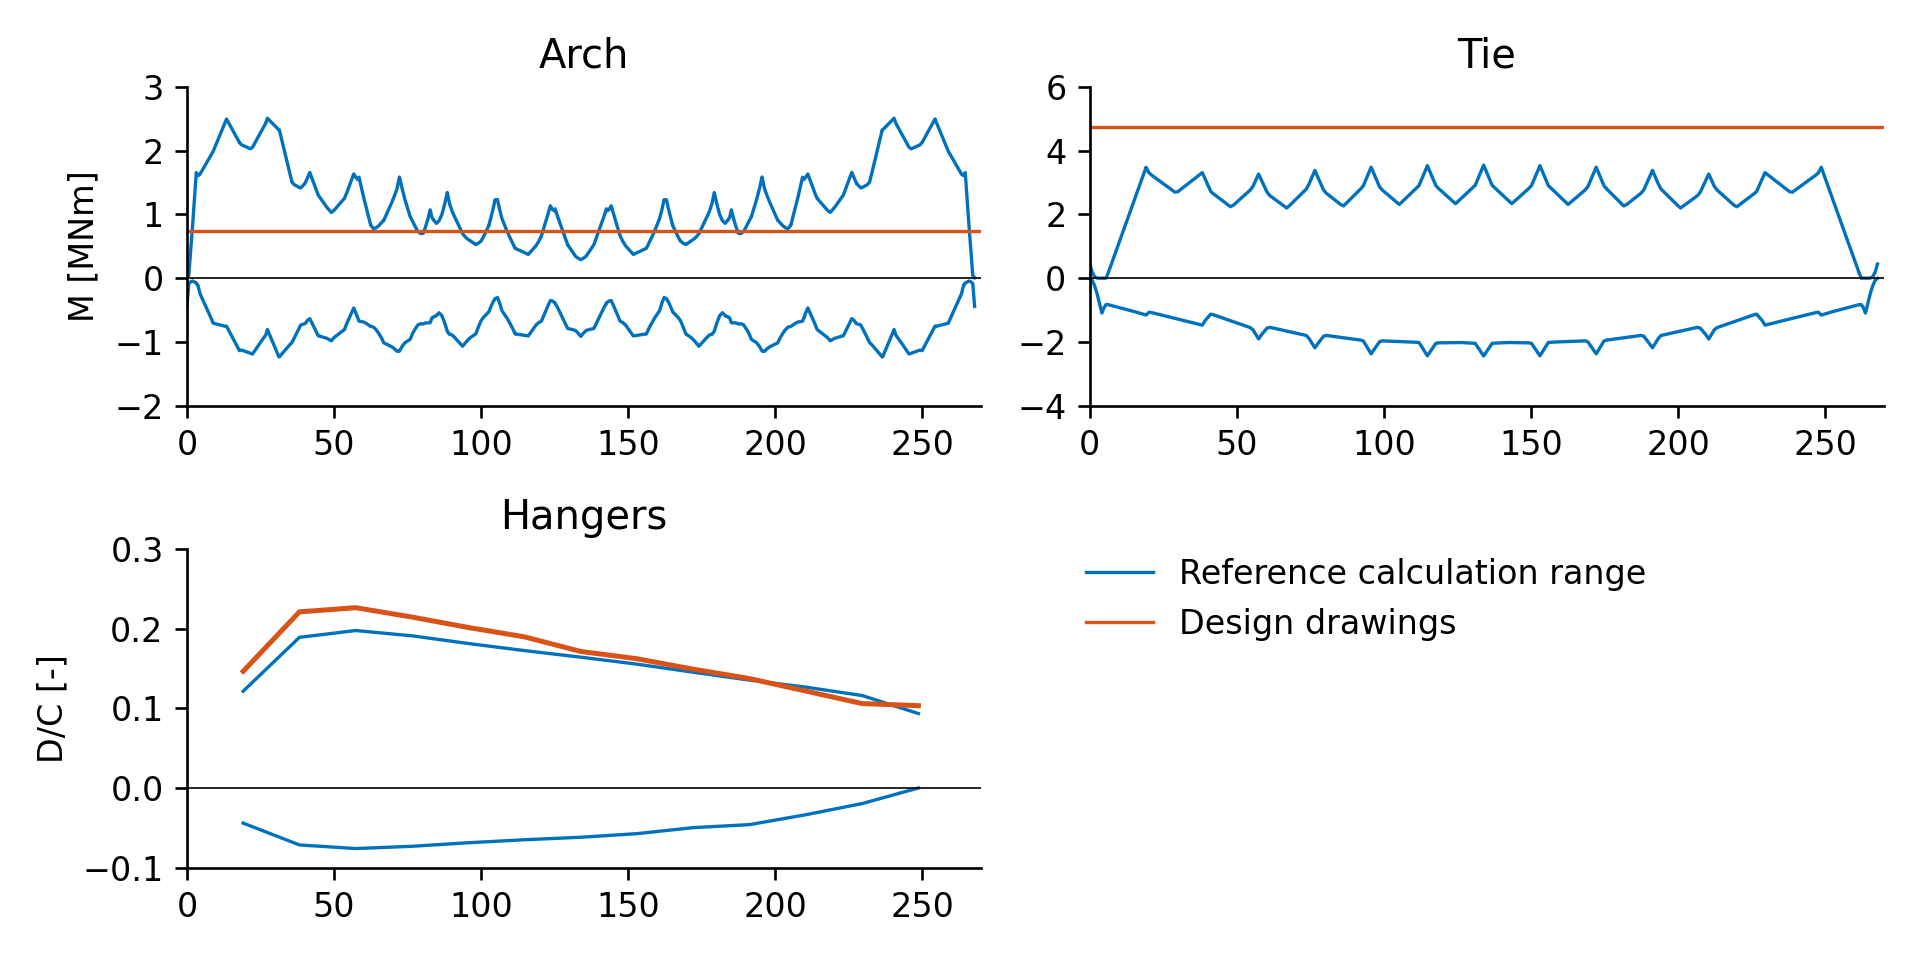
\includegraphics[width=0.8\textwidth]{calculations/Base case/Live load.png}
    \caption{Range of internal forces effects under live loading}
    \label{fig:base_case_live}
\end{figure}

Apparently, the moments in the arch which are given in the design drawings do not correspond to the maximum for the considered load case. The extensive difference cannot be explained in another way and seems physically impossible. The moment distribution in the tie and the normal forces in the hangers seem to agree on the other hand. Apparently, the live loading is only slightly overestimated in the model, which can be seen particularly well in the demand over capacity ratios of the hangers. These differences are accepted, as it is not the goal of this Thesis to reproduce the results from the design drawings. Interestingly, in particular the arch segment near the knuckle is affected by strong bending moments. In the tie girder on the other hand, the possible effects under live loading are well distributed. Apparently, the influence lines for the moments in the tie girder at the different cross-girders follow the same shape. For the hangers, it is the second one from the knuckle connected toward the middle of the arch that undergoes the largest normal force. Towards the other side of the hangers set, the hanger forces decrease. The stronger affected hangers have in common that their inclination is closer to the inclination of the arch at their respective connection node. The arch is very stiff on axial loading and comparably weaker on perpendicular forces. Therefore, at the arch nodes, smaller displacements in direction of the hangers are expected for the strongly affected hangers, explaining their higher normal forces. Only the first hanger does not follow this rule, which can be explained by its smaller area of influence. \medskip